%%%%%%%%%%%%%%%%%%%%%%%%%%%%%%%%%%%%%%%%%%%%%%%%%%%%%%%%%%%%%%%%%%%%%%%%%%%%%%%%
%2345678901234567890123456789012345678901234567890123456789012345678901234567890
%        1         2         3         4         5         6         7         8

\documentclass[letterpaper, 10 pt, conference]{ieeeconf}  % Comment this line out
                                                          % if you need a4paper
%\documentclass[a4paper, 10pt, conference]{ieeeconf}      % Use this line for a4
                                                          % paper

\IEEEoverridecommandlockouts                              % This command is only
                                                          % needed if you want to
                                                          % use the \thanks command
\overrideIEEEmargins
% See the \addtolength command later in the file to balance the column lengths
% on the last page of the document



% The following packages can be found on http:\\www.ctan.org
%\usepackage{graphics} % for pdf, bitmapped graphics files
%\usepackage{epsfig} % for postscript graphics files
%\usepackage{mathptmx} % assumes new font selection scheme installed
%\usepackage{times} % assumes new font selection scheme installed
%\usepackage{amsmath} % assumes amsmath package installed
%\usepackage{amssymb}  % assumes amsmath package installed
\usepackage{standalone} % for including tikz documents
\usepackage{tikz}
\usepackage{listings}

\title{\LARGE \bf
Automated Three Vessel Home Brewing System*
}

%\author{ \parbox{3 in}{\centering Huibert Kwakernaak*
%         \thanks{*Use the $\backslash$thanks command to put information here}\\
%         Faculty of Electrical Engineering, Mathematics and Computer Science\\
%         University of Twente\\
%         7500 AE Enschede, The Netherlands\\
%         {\tt\small h.kwakernaak@autsubmit.com}}
%         \hspace*{ 0.5 in}
%         \parbox{3 in}{ \centering Pradeep Misra**
%         \thanks{**The footnote marks may be inserted manually}\\
%        Department of Electrical Engineering \\
%         Wright State University\\
%         Dayton, OH 45435, USA\\
%         {\tt\small pmisra@cs.wright.edu}}
%}

\author{Alvin Thai$^{1}$ and Nicholas Pelham$^{2}$ \\
	Department of Computer Science and Engineering \\
    University of California - Riverside \\
    \tt\small athai005@ucr.edu npelh001@ucr.edu
\thanks{*The system is simulated. No alcoholic beverages were made during the course of this project, but some were consumed.}% <-this % stops a space
\thanks{$^{1}$A. Thai is a Senior Computer Engineering Major who is too young to have as yet enjoyed a good beer}%
\thanks{$^{2}$N. Pelham is a Senior Computer Engineering Major with a decade of experience in and around the San Diego craft beer industry}%
}


\begin{document}



\maketitle
\thispagestyle{empty}
\pagestyle{empty}


%%%%%%%%%%%%%%%%%%%%%%%%%%%%%%%%%%%%%%%%%%%%%%%%%%%%%%%%%%%%%%%%%%%%%%%%%%%%%%%%
\begin{abstract}

Brewing beer at home is a popular hobby of craft beer enthusiasts. In this paper, we layout the requirements and designs for our proposed system to automate the process of creating wort, the sugary liquid extract which is fermented into beer. The fermentation process is not considered here, as it involves storing the wort and yeast mixture for several weeks until fermentation is complete. 

Automating the home brewing process reduces the risk of infection, improving the quality of the finished brew; and reduces the barrier to entry caused by the complexities in the process, allowing people to more easily enter the home brewing markets.

\end{abstract}


%%%%%%%%%%%%%%%%%%%%%%%%%%%%%%%%%%%%%%%%%%%%%%%%%%%%%%%%%%%%%%%%%%%%%%%%%%%%%%%%
\section{INTRODUCTION}

The majority of small batch home brewing is accomplished using recipe kits containing malt extract, which greatly limits the brewers' available creative options. The alternative method, all grain brewing, allows for greater opportunities to create unique brews. The process requires two additional vessels, additional ingredients, a noticeable amount of additional work.

Malt extract brewing is accomplished with a single vessel. Water is brought to a boil for a certain amount of time, and ingredients are added at various specified times within the boil at the end of which the wort is chilled either by allowing the mixture to sit until it's temperature falls to a specified temperature, by submerging the vessel in an ice bath, or by use of an immersion chiller.

In contrast, all grain brewing is accomplished most frequently with three vessels. Water is brought to a desired temperature within the first vessel, referred to as the Hot Liquor Tank. The Hot Liquor Tank's purpose is to bring water to a required temperature to be added to the Mash Tun, the second vessel. The Mash Tun is where the process of extracting malt sugars from grains is done by allowing the grains to soak within heated water until the starch within the grain is converted naturally to sugars. The water, now high in sugar content, is then moved into the final vessel in the process: the Boil Kettle. The Boil Kettle is in effect the single vessel used in malt extract brewing, and the process is similar with the difference of not requiring malt extract, syrups, or sugars to be added.

\section{MECHANICAL SYSTEM DESIGN}

The goal of our mechanical system design is to reduce the cost of the final product by utilizing parts within the system to accomplish multiple tasks. To this effect, we have chosen a single pump design which uses solenoid valves to direct the flow of liquid between all three vessels. A single heat exchange coil is used both for a heat exchange recirculating mash system (HERMS), and as an immersion chiller to crash cool the finished wort. The drawback of the system is that a single pump limits the systems ability to continuously sparge the mash, forcing a psuedo fly sparge to be implemented instead.

\begin{figure}[!htb]
  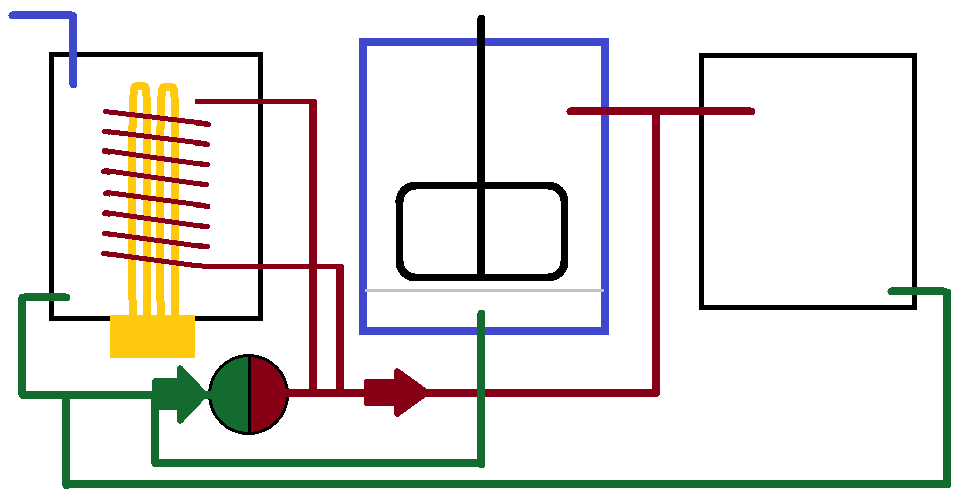
\includegraphics[width=0.5\textwidth]{3vbs}
  \caption{Mechanical System Design}
\end{figure}

The following paragraph is a description of fig 1. The goal of our mechanical system design is to reduce the cost of the final product by utilizing parts within the system to accomplish multiple tasks. To this effect, we have chosen a single pump design which uses solenoid valves to direct the flow of liquid between all three vessels. A single heat exchange coil is used both for a heat exchange recirculating mash system (HERMS), and as an immersion chiller to crash cool the finished wort. The drawback of the system is that a single pump limits the systems ability to continuously sparge the mash, forcing a psuedo fly sparge to be implemented instead.

\section{COMPLEXITIES}

The complexity involved in our design comes largely from utilizing multiple ATMega1284 controllers, a requirement for the Intermediate Embedded Systems course which this system is designed within. A single ATMega is used to control each individual vessel, each connected through SPI to a single master which controls the transportation mechanisms and acts as an interface through which a user operates the system. The synchronization of all of these tasks is expected to fulfill most of the assignment's complexity requirements.

Hardware complexities include thermal resistors used to monitor the temperature within each vessel, liquid flow meters to monitor the amount of liquid entering the hot liquor tank and the boil kettle, and float switches to monitor the level of the mash tun. Additionally, and time permitting, an LCD touchscreen will be implemented on the master controller as a user interface through which all processes will be controlled, and all variables will be displayed.

\section{LIMITATIONS}

Because of limited time, funding being provided exclusively by ourselves, and the focus of the course for which this product is being developed; several key components will not be included in the product presented at the end of the course. These include all physical vessels, pipes, valves, heaters, and the pump. Valves and heaters will be simulated using LEDs, the pump will be simulated using a DC motor, and the stirring motor for the mash tun will be simulated with a smaller stepper motor.

The initial prototype used for testing will make use of several available parts which function similar to the parts expected to be included in the graded project. In the event that the parts are not delivered in a timely manner, the simulated parts will be used in the presentation. These parts include: potentiometers in place of thermal resistors, mechanical switches in place of float switches, and software timers in place of flow sensors.

\section{PRODUCT PRESENTATION}

The final presentation for the course will be done using primarily simulated parts. A drawing, or other mock up available at the time of the presentation, will be displayed with LEDs, a stepper motor, and a DC motor in appropriately visible locations so as to demonstrate the desired functionality of the product. Timers will be set to appropriately short intervals so as to complete the demonstration in a timely manner.

\section{STATE MACHINE DESIGN}

\subsection{Hot Liquor Tank}

Lorem ipsum dolor sit amet, consectetur adipiscing elit, sed do eiusmod tempor incididunt ut labore et dolore magna aliqua. Ut enim ad minim veniam, quis nostrud exercitation ullamco laboris nisi ut aliquip ex ea commodo consequat. Duis aute irure dolor in reprehenderit in voluptate velit esse cillum dolore eu fugiat nulla pariatur. Excepteur sint occaecat cupidatat non proident, sunt in culpa qui officia deserunt mollit anim id est laborum.

\begin{figure}[!htb]
  \centering
  \includestandalone[mode=buildnew]{HLT_SM}
  \caption{Hot Liquor Tank State Machine}
\end{figure}

\subsection{Mash Tun}

Lorem ipsum dolor sit amet, consectetur adipiscing elit, sed do eiusmod tempor incididunt ut labore et dolore magna aliqua. Ut enim ad minim veniam, quis nostrud exercitation ullamco laboris nisi ut aliquip ex ea commodo consequat. Duis aute irure dolor in reprehenderit in voluptate velit esse cillum dolore eu fugiat nulla pariatur. Excepteur sint occaecat cupidatat non proident, sunt in culpa qui officia deserunt mollit anim id est laborum.

\begin{figure}[!htb]
  \centering
  \includestandalone[mode=buildnew]{MT_SM}
  \caption{Mash Tun State Machine}
\end{figure}

\subsection{Boil Kettle}

Lorem ipsum dolor sit amet, consectetur adipiscing elit, sed do eiusmod tempor incididunt ut labore et dolore magna aliqua. Ut enim ad minim veniam, quis nostrud exercitation ullamco laboris nisi ut aliquip ex ea commodo consequat. Duis aute irure dolor in reprehenderit in voluptate velit esse cillum dolore eu fugiat nulla pariatur. Excepteur sint occaecat cupidatat non proident, sunt in culpa qui officia deserunt mollit anim id est laborum.

\begin{figure}[!htb]
  \centering
  \includestandalone[mode=buildnew]{BK_SM}
  \caption{Boil Kettle State Machine}
\end{figure}

\section{SPI PROTOCOLS}

All SPI communication is done by passing a \texttt{struct SPI\_Data} filled with the both useful data, and null data used to conform to a single communication standard between all functions. The function \texttt{void handleReceivedData(void)} is defined for each component to handle receiving the data differently.

\begin{figure}[thpb]
\begin{center}
\begin{tabular}{|c|}
\hline
\begin{lstlisting}
struct SPI_Data {
    unsigned char  flag;
    unsigned short temp;
    signed   short time;
    unsigned short vol;
}
\end{lstlisting} \\
\hline
\end{tabular}
\end{center}
\caption{Data type used for SPI communication}
\end{figure}

\section{CONCLUSIONS}

A conclusion section is not required. Although a conclusion may review the main points of the paper, do not replicate the abstract as the conclusion. A conclusion might elaborate on the importance of the work or suggest applications and extensions. 

\addtolength{\textheight}{-12cm}   % This command serves to balance the column lengths
                                  % on the last page of the document manually. It shortens
                                  % the textheight of the last page by a suitable amount.
                                  % This command does not take effect until the next page
                                  % so it should come on the page before the last. Make
                                  % sure that you do not shorten the textheight too much.

%%%%%%%%%%%%%%%%%%%%%%%%%%%%%%%%%%%%%%%%%%%%%%%%%%%%%%%%%%%%%%%%%%%%%%%%%%%%%%%%



%%%%%%%%%%%%%%%%%%%%%%%%%%%%%%%%%%%%%%%%%%%%%%%%%%%%%%%%%%%%%%%%%%%%%%%%%%%%%%%%



%%%%%%%%%%%%%%%%%%%%%%%%%%%%%%%%%%%%%%%%%%%%%%%%%%%%%%%%%%%%%%%%%%%%%%%%%%%%%%%%
\section*{APPENDIX}

Appendixes should appear before the acknowledgment.

\section*{ACKNOWLEDGMENT}

The preferred spelling of the word ÒacknowledgmentÓ in America is without an ÒeÓ after the ÒgÓ. Avoid the stilted expression, ÒOne of us (R. B. G.) thanks . . .Ó  Instead, try ÒR. B. G. thanksÓ. Put sponsor acknowledgments in the unnumbered footnote on the first page.



%%%%%%%%%%%%%%%%%%%%%%%%%%%%%%%%%%%%%%%%%%%%%%%%%%%%%%%%%%%%%%%%%%%%%%%%%%%%%%%%

References are important to the reader; therefore, each citation must be complete and correct. If at all possible, references should be commonly available publications.



\begin{thebibliography}{99}

\bibitem{c1} G. O. Young, ÒSynthetic structure of industrial plastics (Book style with paper title and editor),Ó 	in Plastics, 2nd ed. vol. 3, J. Peters, Ed.  New York: McGraw-Hill, 1964, pp. 15Ð64.






\end{thebibliography}




\end{document}
